\documentclass{standalone}
\usepackage{pgfplots}
\usepackage{xcolor}
\begin{document}
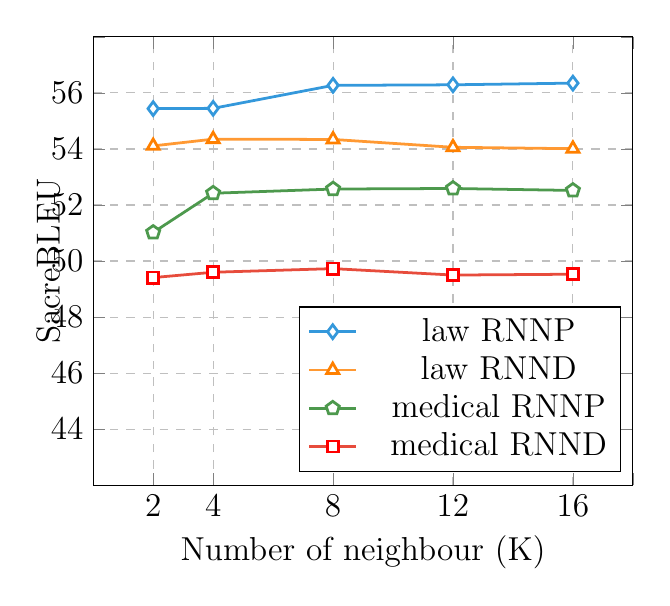
\begin{tikzpicture}
\definecolor{upurple}{RGB}{155,89,182}
\definecolor{ublue}{RGB}{52,152,219}
\definecolor{ured}{RGB}{231,76,60}
\definecolor{udark}{RGB}{77,153,77}
\definecolor{ugreen}{RGB}{46,204,113}
% 设置第一个图表的样式
\begin{axis}[
name=plot1, % 图表名称
at={(0,0)}, % 设置图表的位置
xshift=-3cm, % 向左移动3cm
ymajorgrids, % 主要网格线
xmajorgrids, % 主要网格线
grid style=dashed, % 网格线样式
legend style={
at={(0.68,0.03)},
anchor=south,
legend columns=1,
column sep=2.27ex,
font={\large},
%draw=none,
}, % 图例位置
xlabel={\large Number of neighbour (K)}, % X轴标签
ylabel={\large SacreBLEU}, % Y轴标签
ylabel style={yshift=-1em}, % Y轴标签偏移
xlabel style={yshift=0em}, % X轴标签偏移
%yticklabel style={/pgf/number format/precision=1, /pgf/number format/fixed zerofill, font={\Huge}}, % Y轴刻度标签格式
ymin=42, ymax=58, % Y轴范围
ytick={42,44,46,48,50,52,54,56,58},
yticklabels={,44,46,48,50,52,54,56,},
xmin=0, xmax=18, % X轴范围
xtick={2,4,8,12,16,18}, % X轴刻度
xticklabels={2,4,8,12,16,},
xticklabel style={font={\large}}, % X轴刻度标签格式
yticklabel style={font={\large}} % X轴刻度标签格式
]

\addplot[ublue,mark=diamond*,mark size=2.5pt,line width=1pt,mark options={fill=white,draw=ublue,line width=1pt}]
coordinates {(2,55.44) (4,55.45) (8,56.27) (12,56.29) (16,56.35)};
\addlegendentry{law RNNP}

% 绘制第一个图表的数据系列
\addplot[orange!80,mark=triangle*,mark size=2.5pt,line width=1pt,mark options={fill=white,draw=orange,line width=1pt}]
coordinates {(2,54.11) (4,54.35) (8,54.34) (12,54.06) (16,54.01)};
\addlegendentry{law RNND}

\addplot[udark,mark=pentagon*,mark size=2.5pt,line width=1pt,mark options={fill=white,draw=udark,line width=1pt}]
coordinates {(2,51.02) (4,52.42) (8,52.57) (12,52.59) (16,52.52)};
\addlegendentry{medical RNNP}

\addplot[ured,mark=square*,mark size=2pt,line width=1pt,mark options={fill=white,draw=red,line width=1pt}]
coordinates {(2,49.41) (4,49.6) (8,49.73) (12,49.5) (16,49.53)};
\addlegendentry{medical RNND}



\end{axis}
\end{tikzpicture}

\end{document}